\documentclass[14pt
%,handout%
]{beamer}

%\usepackage{proof}
\usepackage{mathpartir}

%Beamer configuration

% Include page numbers
\setbeamertemplate{footline}{\hfill\insertframenumber\hspace*{2mm}\vspace*{2mm}}

\usetheme{Pittsburgh}

% switch off the fancy navigation symbols
\setbeamertemplate{navigation symbols}{}

\setbeamertemplate{section in toc}[ball unnumbered]

%\usefonttheme[onlymath]{serif}
%\usepackage{tikz}
%\usetikzlibrary{matrix}
%\usetikzlibrary{shapes.geometric}

\definecolor{darkblue}{rgb}{0.0,0.0,0.5}
\newcommand<>{\high}[1]{{\color#2{blue}{#1}}}
\newcommand<>{\bad}[1]{{\color#2{red}{#1}}}
\newcommand{\gray}[1]{\textcolor{gray}{#1}}

\newcommand{\concept}[1]{\high{\emph{#1}}}
\newcommand{\important}{{\Large \textbf{!}}}

\newcommand<>{\altvphantom}[2]{\alt#3{#1}{#2}\vphantom{#1}\vphantom{#2}}

%%%%%%%%%%%%%%%%%%%%%%%%%%%%%%%%%%%%%%%%%%%%%%%%%%%%%%%%%%%%%%%%%%%%%%%%%%%%%%%

\AtBeginSection[]
{
\begin{frame}
\setcounter{tocdepth}{1}
\tableofcontents[currentsection]
\end{frame}
}
\AtBeginSubsection[]
{
\begin{frame}
\setcounter{tocdepth}{2}
\tableofcontents[sectionstyle=show/hide,subsectionstyle=show/shaded/hide]
\end{frame}
}

\begin{document}

\title{Verification of Earley's Algorithm \\ Including Time Bounds}
\author{Tobias Nipkow, Alexander Haberl}
\institute[]{%
	Technische Universit\"at M\"unchen\\ \vspace{1cm}
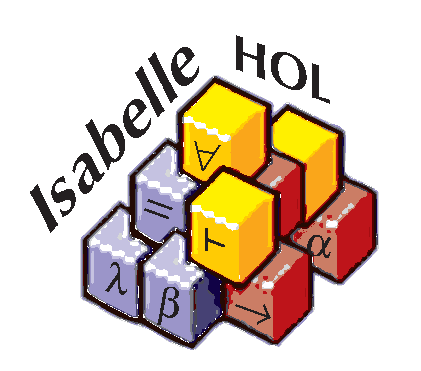
\includegraphics[scale=.4]{isabelle_hol}}
\date{}%\the\year-\the\month-\the\day}
\maketitle

%-------------------------------------------------------------
\section{Background}
%-------------------------------------------------------------
\begin{frame}{Earley's Algorithm}
\framesubtitle{PhD 1968, CACM 1970}
\pause
Earley's algorithm:\\\quad Parser for all context-free grammars
\bigskip\pause

Earley's \emph{recognizer}:\\\quad Decision procedure, no parse trees
\end{frame}
%-------------------------------------------------------------
\begin{frame}{Usually defined imperatively}
Initialize $E_0, \dots, E_n$ to $\emptyset$
\pause

for $i = 0$ to $n$ do\\
\quad Process the $s \in E_i$ \emph{in order}:\pause\\
\qquad If \dots\ then \high{add \dots\ to $E_i$}\\
\qquad If \dots\ then \high{add \dots\ to $E_{i+1}$}
\end{frame}
%-------------------------------------------------------------
\begin{frame}{Some early proofs}
%\begin{itemize}
\pause

%\item
"By induction on the number of items added to any item set
before \dots\ is added to $E_i$"\pause\smallskip\\ (Earley)
\pause\bigskip

%\item
``The rank is computed as follows:\pause\\
Let $a$ be the length of a shortest derivation $\dots$\\
Let $b$ be the length of a shortest derivation $\dots$\\
Let $c$ be the length of a shortest derivation $\dots$\pause\\
The rank is defined as \high{$a + 2(j + b + c)$'}'\pause\smallskip\\
(Aho \& Ullman)
%\end{itemize}
\end{frame}
%-------------------------------------------------------------
\begin{frame}{Cliff Jones: Fixpoints!}
\framesubtitle{1971}
\pause
Define each $E_{i+1}$ as least fixpoint\\ (closure under Scan, Predict, Complete)\pause\\
depending on $E_0$, \dots, $E_i$
\pause\bigskip

2 nested fixpoints
\pause\bigskip

Proofs by fixpoint inductions
\end{frame}
%-------------------------------------------------------------
\begin{frame}{\mbox{First$^?$ recognizer verification:} Obua 2017}
\begin{itemize}
\pause
\item
Based on Jones
\pause
\item Complicated
\end{itemize}
\end{frame}
%-------------------------------------------------------------
\begin{frame}{\mbox{First$^?$ parser verification:} \mbox{Rau \& N.\ 2023/24}}
\begin{itemize}
\pause
\item
Based on Obua
\pause
\item The parser complication:\\ representing and extracting\\ the
  (possibly infinite) set of parse trees\pause\\
  Correctness proved only for a single parse tree
\pause
\item Even the recognizer is complicated
\pause
\item Can we simplify it?
\end{itemize}
\end{frame}
%-------------------------------------------------------------
\section{Abstract Earley}
%-------------------------------------------------------------
\begin{frame}
\textbf{Input}: Grammar $G$, input word $w=a_0\dots a_{n-1}$
\medskip\pause

Earley generates sets $E_0, \dots, E_n$ of \high{\emph{items}} \pause
\begin{center}
\high{$(A \to \alpha\bullet\beta, i)$}
\end{center} \pause

Aim: \[ (A \to \alpha\bullet\beta, \bad{i}) \in E_{\high{j}} \quad \text{iff} \quad \alpha \to_G^* a_{\bad{i}} \dots
  a_{\high{j}-1} \]
\end{frame}
%-------------------------------------------------------------
\begin{frame}{Inductive Definition of $E_i$}
\[ \high<1>{\inferrule{(S \to \alpha) \in G}{(S \to \bullet\alpha,0) \in E_0}}{\textsc{Init}}\]
\pause
\[ \inferrule{\high<2>{(A \to \fbox{$\alpha\bullet a_j \beta$}, i) \in E_j}}
  {\pause\high<3>{(A \to \fbox{$\alpha a_j\bullet \beta$}, i) \in E_{j+1}}}{\textsc{Scan}}
\]
\pause
\[ \inferrule{\high<4>{(A \to \fbox{$\alpha\bullet B \beta$}, i) \in E_j} \\\pause \high<5>{(B \to \gamma) \in G}}
  {\pause\high<6>{(B \to \bullet \gamma, j) \in E_j}}{\textsc{Predict}}
\]
\pause
\[ \hspace{-1em}\inferrule{ \high<7>{(B \to \fbox{$\gamma\bullet$}, i) \in E_j} \\\pause \high<8>{(A \to
    \fbox{$\alpha \bullet B \beta$}, k) \in E_i}}
  {\pause\high<9>{(A \to \fbox{$\alpha B \bullet \beta$}, k) \in E_j}}{\textsc{Complete}}
\]
\end{frame}
%-------------------------------------------------------------
% \begin{frame}
%   \begin{center}
% Similar description found in MSc thesis\\by Elias Forsberg (supervised
% by Andreas Abel)
%     \end{center}
% \end{frame}
%-------------------------------------------------------------
\begin{frame}{Soundness easy}
\[ (A \to \alpha\bullet\beta,i) \in E_j \ \Longrightarrow \ \alpha \to_G^*
  a_i\dots a_{j-1} \]
\pause\bigskip

Proof by induction on the definition of $E_j$
\end{frame}
%-------------------------------------------------------------
\begin{frame}{Completeness}
\[ S \to_G^* w \ \Longrightarrow\ \exists (S\to\alpha)\in G.\ (S \to \alpha\bullet, 0) \in E_n \]
\bigskip\pause

Proof: generalization(!) and two nested inductions\pause\\ (length
of derivation, length of rhs)
\end{frame}
%-------------------------------------------------------------
\section{Stepwise Refinement}
%-------------------------------------------------------------
\begin{frame}
  \begin{center}
    The refinement proofs are standard\\
    if we do not comment on them
  \end{center}
\end{frame}
%-------------------------------------------------------------
\subsection{Standard Earley}
%-------------------------------------------------------------
\begin{frame}
  Fact: $E_j$ depends only on $E_i$ where $i \le j$
  \pause\medskip
  
  Define $E_0, \dots, E_n$ one after the other\\
  depending only on previous and current item sets
  \pause\medskip
  
  Implementation: growing list of \high{bins} = items sets: $\textbf{B}_j = [B_0,\dots,B_j]$
  \pause\medskip
  
Recursive definition:\pause\smallskip
  
$\textbf{B}_0 = [close\ []\ Init]$\pause

$\textbf{B}_{j+1} = \textbf{B}_j\; @\; [close\;\textbf{B}_j\;(Scan(last(\textbf{B}_j)))]$
  \pause\medskip
  
  $close\; \textbf{B}_j\;B$ = closure of $B$\\ under \textsc{Predict} and \textsc{Complete}
  wrt $\textbf{B}_j$
  \pause\medskip
  
\textbf{Thm} $\textbf{B}_n = [E_0,\dots E_n]$
\pause\medskip

Refinement focuses on \high{closure} from now on
\end{frame}
% -------------------------------------------------------------
\subsection{Epsilon}
%-------------------------------------------------------------
\begin{frame}{A complication due to \textsc{Complete}}
 \bad{$close \;\textbf{B}_j \;B$ \ may need to combine two elements of $B$}\pause\\
 but only \bad{if the grammar has $\epsilon$ productions}
 \pause
 \begin{center}
  \high{We assume that the grammar is $\epsilon$-free}
  \pause
  \end{center}

  Now we can combine \textsc{Predict} and \textsc{Complete}
  into a single function\\ \high{$PreCo :: bins \to item \to item\; set$}
  \pause\bigskip
  
  Closure is saturation under $PreCo$.
\end{frame}
%-------------------------------------------------------------
\subsection{Work set algorithm (inductive)}
%-------------------------------------------------------------
\begin{frame}{$(B,C) \to (B',C')$}
  $B,C:: item\; set$\\
  $B$: to be visited (work set), $C$: visited
  \bigskip\pause
  
  One $Step$ (eg $PreCo$):
  \medskip\pause
  
  \[ \inferrule{x \in B \quad C' = C \cup \{x\}
      \quad B' = (B\setminus\{x\}) \cup (Step\;x  \setminus C')}
    {(B,C) \to (B', C')} \]
  \pause
  $closure~B = SOME\ C.\ (B,\{\}) \to^* (\{\},C)$
\end{frame}
%-------------------------------------------------------------
\subsection{Work list algorithm (inductive)}
%-------------------------------------------------------------
\begin{frame}{$(B,C) \to_L (B',C')$}
  $B,C$: item list

  Pick first element of $B$ in every step
\end{frame}
%-------------------------------------------------------------
\subsection{Recursive}
%-------------------------------------------------------------
\begin{frame}{}
  $close\;([],C) = Some\;C$\\
  $close\;(x\#B,C) =$\\
  \qquad$close\; (let \;C' = \dots; B' = \dots\;in\ (B',C'))$
   \pause
  \begin{center}
    \high{An executable algorithm!}
  \end{center}
 \pause
  
  Why $Some$? \pause\smallskip To signal definedness/termination!
  \pause\smallskip
  
  Otherwise $None$ \pause\smallskip
  
  Needed because $close$ is a partial function:\\ input $(B,C)$ may not be wellformed.
  \pause\medskip
  
  \textbf{Thm} $close$ yields $Some$ for wellformed inputs.
\end{frame}
%-------------------------------------------------------------
\section{Parser}
%-------------------------------------------------------------
\begin{frame}
  Instrument recognizer with parse trees\pause\bigskip
  
  Only 1 parse tree!\\
  Only useful for unambiguous grammars

\end{frame}
%-------------------------------------------------------------
\section{Complexity}
%-------------------------------------------------------------
\begin{frame}{Space complexity}
  Grammar is fixed! \pause\\
  $\Longrightarrow$ only a fixed number of dotted rules
  \pause\medskip
  
Input size $n = |w|$ \pause\medskip

Remember: item $(A \to \alpha\bullet\beta, i)$ where $i \le n$
\pause\smallskip

$\Longrightarrow$ Size of each bin $O(n)$
\pause\bigskip

If we partition each bin by the from-index $i$\\
each partition has size $O(1)$

\end{frame}
%-------------------------------------------------------------
\begin{frame}{Time complexity}
  Problem: in each closure step,\\ need to remove $B$ and $C$  from
  the ``new'' items \pause
  
  Hence the set (list) difference
  \begin{itemize}
    \pause
  \item set difference is $O(n^2)$ with linear search
    \pause
  \item the construction of each bin takes $O(n)$ steps
    \pause
  \item there are $n$ bins
  \end{itemize}
  \pause
  \bad{$= O(n^4)$} \pause
  \begin{center}
  \bad{Need to improve set difference}
\end{center}
\end{frame}
%-------------------------------------------------------------
\begin{frame}{Bins as functions}
  Assume bins are functions:: from-index $\to$ item list\pause\\
  Then each item list has size $O(1)$ \pause\medskip

  Assume access $bin(i)$ takes time $T_B$ \pause\medskip

  Then searching for $(A \to \alpha\bullet\beta,i)$  takes time
  $T_B(n)$\pause\medskip

  Possible implementations of bins:
  \begin{itemize}
  \item list: $T_B$ is linear
  \item tree: $T_B$ is logarithmic
  \item array: $T_B$ is constant
\end{itemize}
\end{frame}
%-------------------------------------------------------------
\begin{frame}{Time complexity, verified}
\begin{center}
\large\high{ $O(n^3\cdot T_B(n))$}
\end{center}
\end{frame}
%-------------------------------------------------------------
\begin{frame}{Infrastructure}
  \begin{center}
  \high{Automatic generation of $T_f$ from $f$}\pause\\
  Unverified
\end{center}
\pause
Alternative: write all functions in a time monad
\end{frame}
%-------------------------------------------------------------
\begin{frame}{Method}
  \begin{center}
    \high{Prove closed upper bounds for $T_f$ by induction}\pause\\
    \bad{Upper bounds with ugly constants}\pause\\
    \bad{Maintenance hell!}
\end{center}
\end{frame}
%-------------------------------------------------------------
\begin{frame}{Presentation}
  \begin{center}
    Thin layer of $T_f \in O(.)$ lemmas\\derived from the concrete bounds
\end{center}
\end{frame}
%-------------------------------------------------------------
\begin{frame}{Size of formalization}
  \begin{tabular}{lrr}
    & Refinement & Time\\
 Recognizer: & 2000 & 1000\\
 Parser: & 1000 & 1000
\end{tabular}
\end{frame}
%-------------------------------------------------------------
\begin{frame}{Better:\\ Reasoning directly with $O$}
  \pause
  Just proved:
  \bigskip
  
  \textbf{Lemma}
  If $f(n+1) = f(n) + g(n)$\pause\\
  and $g \in O(\lambda n.\ n^k)$\pause\\
  then $f \in O(\lambda n.\ n^{k+1})$
  \bigskip\pause
  
  TODO: Apply it!
\end{frame}
%-------------------------------------------------------------
\end{document}